\documentclass[11pt, a4paper]{article}
\usepackage[a4paper, top=2.5cm, bottom=2.5cm, left=2.5cm, right=2.5cm]{geometry}

\usepackage{fontspec}
\usepackage[spanish, english]{babel}
\babelfont{rm}{Noto Sans}
\selectlanguage{spanish}

\usepackage{enumitem}
\setlist[itemize]{label=-}

\usepackage{amsmath,amssymb}
\usepackage{booktabs}
\usepackage{siunitx}
\DeclareSIUnit\mmHg{mmHg} % Define mmHg para evitar warning
\usepackage{graphicx}
\usepackage[hidelinks]{hyperref}
\usepackage{xcolor}

% Añadir ruta de búsqueda de imágenes
\graphicspath{{reports/}{./}}

\title{Proyecto AASIM - Fase 1: Diseño y Planificación \\ \large Estimación Continua de Presión Arterial vía ECG}
\author{Equipo E (Juan Manuel Buitrago, Luis Carlos Rocha, German Alberto Hidalgo)}
\date{\today}

\begin{document}
\maketitle

\begin{abstract}
El presente documento detalla la Fase 1 (Diseño y Planificación) del proyecto AASIM. El problema central radica en que los monitores de presión arterial tradicionales (de manguito) generan "puntos ciegos clínicos", impidiendo un monitoreo continuo y proactivo de la hipertensión (principal factor de riesgo cardiovascular). Se propone el diseño de un Software como Dispositivo Médico (SaMD) basado en IA para estimar la presión arterial a partir de señales de ECG. Este informe define la estructura PICO, las métricas de éxito, los requisitos de los stakeholders y los protocolos de gobernanza de datos necesarios para la viabilidad del proyecto.
\end{abstract}

\section{Declaración del Problema y Estructura PICO}
Siguiendo la metodología de estructuración de proyectos clínicos, el problema se define por la necesidad de anticipar crisis hipertensivas 15-30 minutos antes de su ocurrencia, superando las limitaciones físicas de los esfigmomanómetros. La formulación PICO del proyecto es:

\begin{itemize}
    \item \textbf{Población (P):} Adultos con registros simultáneos de ECG y presión arterial, abarcando rangos normotensivos e hipertensivos.
    \item \textbf{Intervención (I):} Sistema automatizado (SaMD) que utiliza Machine Learning sobre variaciones morfológicas y temporales del ECG continuo para predecir la PAS, PAD y PAM.
    \item \textbf{Comparador (C):} Mediciones obtenidas mediante esfigmomanómetros electrónicos validados (\textit{ground truth}).
    \item \textbf{Outcomes (O):} Error absoluto medio (MAE), RMSE, y porcentaje de predicciones dentro de rangos clínicamente aceptables.
    \item \textbf{Tiempo (T):} Ventanas de adquisición de 30 segundos a 5 minutos, validadas en registros independientes.
\end{itemize}

\section{Mapa de Stakeholders y Requisitos}

A continuación se detalla gráficamente la estructura funcional del proyecto, dividida por las áreas principales (Clínica, Ingeniería TI, Ética y Pacientes), evidenciando los requisitos, riesgos y supuestos de cada una.

% Incluir la figura solo si el archivo existe; si no, omitirla sin error
\IfFileExists{reports/Stakeholders_y_requisitos.jpeg}{%
    \begin{figure}[htbp]
        \centering
        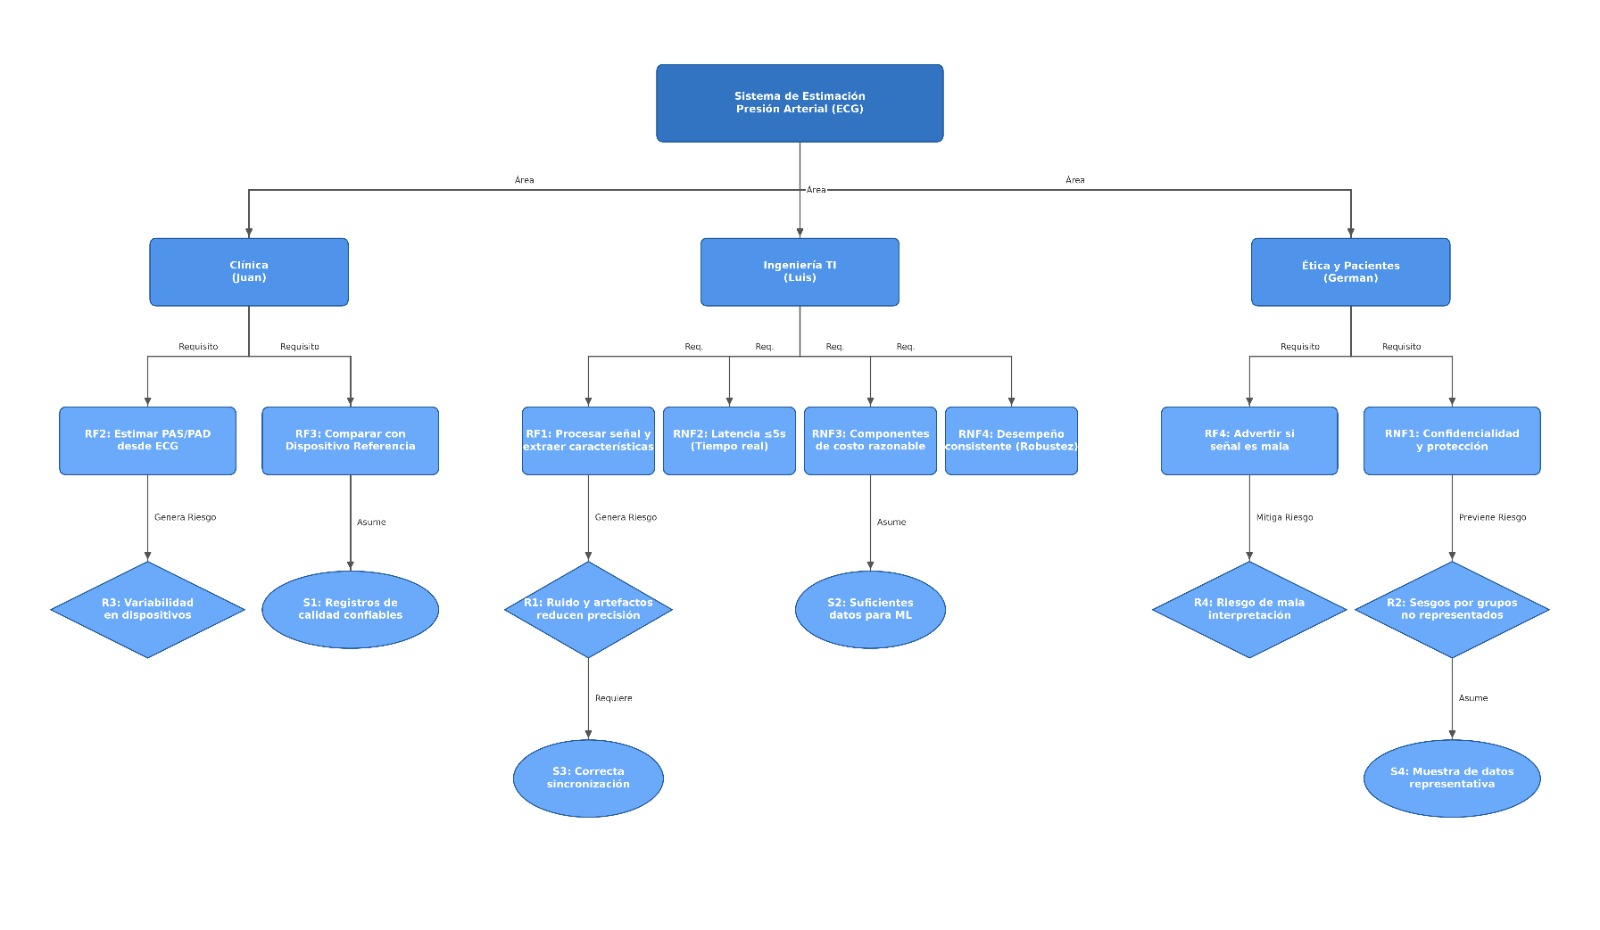
\includegraphics[width=\textwidth]{Stakeholders_y_requisitos.jpeg}
        \caption{Mapa de Stakeholders y Requisitos del sistema AASIM.}
        \label{fig:stakeholders}
    \end{figure}
}{%
    % Si la imagen no está, simplemente no se muestra la figura
    % Puedes incluir un mensaje opcional o dejarlo vacío
}

\section{Plan de Proyecto y Estrategia de Datos}
Para garantizar la validez del modelo a desarrollar, se establece el siguiente plan de gestión de datos y evaluación algorítmica:

\begin{itemize}
    \item \textbf{Datos caracterizados y limpios:} Se extraerán características como la variabilidad de frecuencia cardíaca (HRV). Se controlarán variables de confusión (edad, sexo, medicamentos, postura).
    \item \textbf{Particiones sin fuga (Data Leakage):} Se garantizará que los datos de un mismo paciente no se encuentren simultáneamente en los conjuntos de entrenamiento y validación/prueba.
    \item \textbf{Baseline y SOTA:} El modelo inicial (\textit{baseline}) se basará en regresión lineal sobre el Tiempo de Tránsito del Pulso (PTT). Se comparará con el Estado del Arte (SOTA) en arquitecturas de \textit{Deep Learning} para bioseñales.
\end{itemize}

\section{Indicadores y Criterios de Éxito (Métricas)}

A continuación, se definen los umbrales mínimos que determinarán el éxito técnico y clínico del prototipo.

\begin{table}[htbp]
    \centering
    \caption{Métricas primarias y secundarias propuestas para la evaluación del modelo.}
    \vspace{0.5em}
    \begin{tabular}{llc}
        \toprule
        \textbf{Tipo} & \textbf{Métrica / Indicador} & \textbf{Criterio de Éxito (Umbral)} \\
        \midrule
        Primaria & Error Absoluto Medio (MAE) PAS/PAD & $\le 5$ \unit{\mmHg} \\
        Primaria & Error Cuadrático Medio (RMSE) & $\le 8$ \unit{\mmHg} \\
        Secundaria & Correlación con el comparador (r) & $\ge 0.85$ \\
        Técnica & Latencia de Inferencia (Requisito TI) & $\le 5$ segundos \\
        \bottomrule
    \end{tabular}
    \label{tab:metrics}
\end{table}

\section{Ética, Gobernanza y Plan de Despliegue}
El alineamiento con los stakeholders (Clínica, TI, Ética y Pacientes) exige un marco estricto de cumplimiento:

\begin{enumerate}
    \item \textbf{Evaluación por subgrupos:} Para mitigar el Riesgo R2 (sesgos algorítmicos), las métricas se desglosarán por edad, sexo y comorbilidades. El MAE no debe variar significativamente entre subpoblaciones.
    \item \textbf{Privacidad y Seguridad:} Se aplicarán protocolos de anonimización irreversible a los registros fisiológicos antes de ingresar al \textit{pipeline} de TI, garantizando el RNF1.
    \item \textbf{Plan de despliegue y monitoreo:} El SaMD incluirá un módulo de detección de calidad de señal (RF4). Si el ECG presenta ruido excesivo, el sistema omitirá la predicción en lugar de arrojar falsos positivos, monitoreando continuamente la tasa de rechazo de señales.
\end{enumerate}

\end{document}
